
\section{Monetary Policy}
The Fluidity Protocol is governed through the Fluidity Governance Token. The Fluidity Governance Token facilitates voting on policies while identifying and aligning incentives for the long-term success of the protocol.

\subsection{Tokenomics}
The total supply of Fluid Governance tokens is 1,000,000,000 FLUID tokens, which will be fully circulating no earlier than 4 years post Token Generation Event (TGE.) The token distribution is as follows:

\vspace{1em}
 \begingroup
            \centering{
            \begin{tabular}{||c|c|c||}
            \hline
            \textit{Item} & \textit{Description} & \textit{Percentage} \\\hline
            Seed & Seed Round Investors & \ 13.0\% \\ \hline
            Private & Private Round Investors &\ 5.0\%\\ \hline
            Public & IDO/ IEO &\ 10.0\%\\ \hline
            Community & Utility Mining and Distribution &\ 20.0\%\\ \hline
            Retroactive & Reserved for Airdrops &\ 1.0\%\\ \hline
            DAO & Controlled by Token Holders &\ 26.0\%\\ \hline
            Foundation & Fluidity Foundation and Partners &\ 20.0\%\\ \hline
            Team &Current and Future Team Members&\ 5.0\%\\ \hline
            Sum & &\ 100.0\%\\ \hline

            \end{tabular}}
            \par
\endgroup
           \vspace{1em} 
           
The token emission schedule is as follows:
            
\begin{figure}[h]
    \centering
    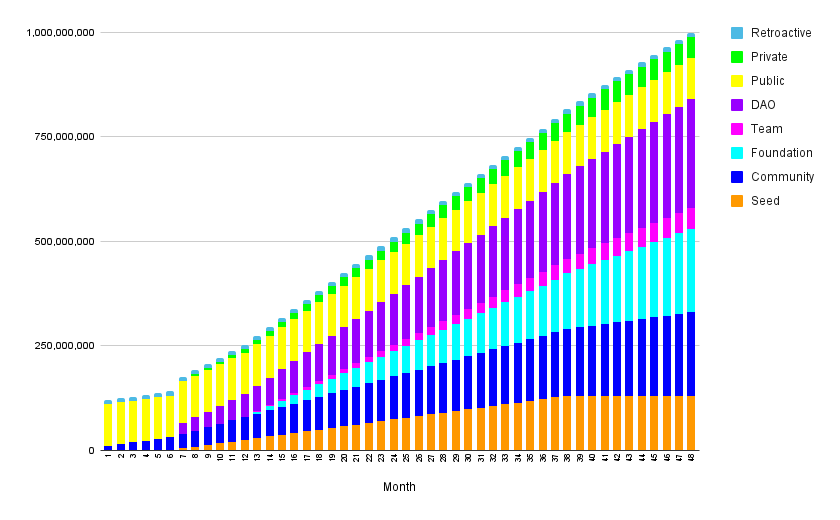
\includegraphics[width=12cm]{images/chart (19).png}
    \caption{Token Emission Schedule}
\end{figure}


\vspace{1em}

\newpage

The Fluidity token supply ownership evolves post-TGE like such:

\begin{figure}[h]
    \centering
    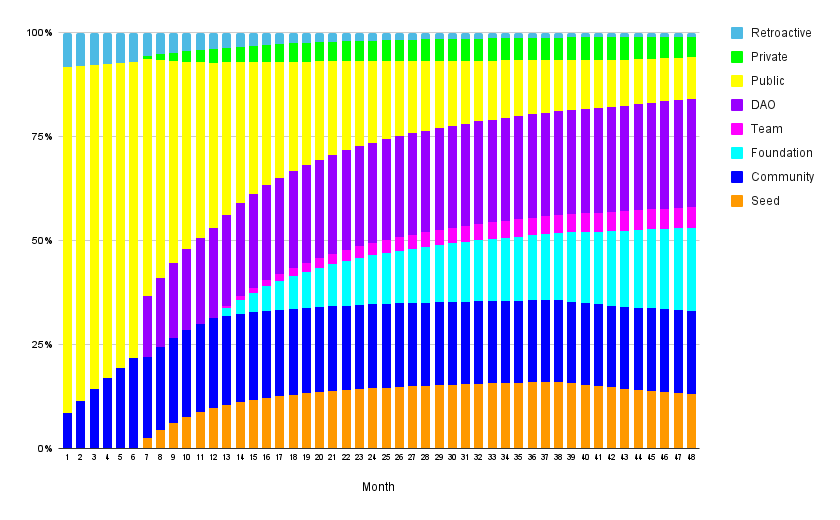
\includegraphics[width=12cm]{images/chart (18).png}
    \caption{Token Emission Schedule}
\end{figure}


\subsection{Token Emission Dilemma and Fluidity}

The objective of the governance token distribution is to maximise diversification amongst genuine users while incentivising positive value creation within the ecosystem. The development of the protocol must be funded and incentives need to be provided to stimulate long-term growth. Much of the funding required to build and grow the protocol, is received and given to a centralised and small number of entities. If these entities have the majority of the circulating supply of governance tokens, they may be able to vote on governance decisions that are favourable to their outcomes over the best interests of the wider ecosystem. Fluidity will minimise and control for this bad behaviour by distributing the majority of the float within the community using its novel Transfer Reward Function distribution.

\subsubsection{Float and Liquidity Mining}
A small float at TGE can inflate the price significantly early, benefiting early insiders. This is unsustainable and misaligns incentives for early token holders, as they will face significant inflation. The protocol faces a dilemma between early and quick growth by introducing a float, or the programmatic distribution of the tokens in a decentralised manner. Liquidity Mining is a method generally employed to increase the float and "hack" the growth of the protocol. Users can accumulate more coins as they enter circulation and actively increase their token holdings with inflation. Much of the liquidity provided in current liquidity mining programs is acquisitive liquidity, as the liquidity providers have no vested interest in the protocol.

 A bonus or lockup with a time multiplier effect can make liquidity more valuable to the protocol. One potential strategy is to introduce Vesting Schedules as a method to reduce selling pressure. However, this model can be improved upon - there is an argument to be made for rewarding active participation in the utility of a protocol, rather than passively participating through liquidity mining and vesting schedules.

Fluidity is exploring a custom model titled Utility Mining that behaves in a manner similar to growth hacking. Users are provided tokens for providing liquidity, but the tokens are vested in a programmatic manner emphasising utility as opposed to time. Utility is defined as the use of Fluid Assets. Liquidity providers will redeem their governance tokens as they use the protocol and engage with the ecosystem proportionate to the amount of liquidity they are providing.

\subsection{Fluidity Governance Token}

Governance is the core of the Fluidity Ecosystem as it provides guidance and structure on determining the size and frequency of payouts, the sources of yield and the token distribution policies. The governance token also entitles the holders to have an increased expected outcome overtime of receiving larger dividends when utilising their Fluid Assets.


\subsubsection{Utility Mining and Distribution}

Fluidity proposes a novel hybrid method to traditional Liquidity Mining programs titled Utility Mining. Although Liquidity Mining will still be utilised, a significant portion of the Fluidity governance tokens will be distributed through Utility Mining. Utility Mining utilises Fluidity's Transfer Reward Function, to provide a fairer mechanism for the distribution of governance tokens, incentivising proactive participation in the protocol and broader ecosystem. 

Utility Mining rewards users with governance tokens and other incentives when they utilise the protocol for intended behaviours. In the Fluidity Protocol, a significant portion of the tokens in the float will be rewarded through utility mining. Utility Mining will ensure that many users understand the functionality and features of Fluidity as participation is necessitated to receive rewards.

\subsubsection{Liquidity as a second order effect of utility}

Utility Mining facilitates organic liquidity within the ecosystem. To participate in Utility Mining, a user must transact with a Fluid Asset. For one to participate in Utility Mining, there must be a liquidity provision event for that specific Fluid Asset. Although one can purchase a Fluid Asset on the open market, significant demand for Fluid Assets will cause a supply shock, only to be redeemed through an increase in minting Fluid Assets. This exchange will generate extra liquidity within the ecosystem. This generates a positive feedback loop, where an increase in the subsequent liquidity causes an increase in utility, as the reward pool grows.

\subsubsection{Broader Ecosystem Participation}
Fluidity increases the utility of assets in the broader ecosystem. By the creation of Fluid Assets, users are now incentivised to utilise their principal rather than holding it idle. By adding modifications to Fluidity's TRF, Fluidity can incentivise participation in value-add use-cases. This includes marketplaces, decentralised exchanges and any use-case where tokens are being transacted on chain. Utility Mining creates an incentive for users to participate in these very use-cases and aligns the communities with genuine participation within the protocol.

\subsubsection{Multiplier effect - Expected Outcome Farming}

As governance token holders have a higher stake in the Fluidity Ecosystem, Fluidity rewards them overtime with a higher Expected Outcome in the form of a multiplier, that increases the exposure to significantly larger dividends when they utilise Fluid assets. This increase in expected outcome can be quantified on a monetary value as it is directly tied to the size of the reward pool and exposure to a larger reward. Eventually Governance Token holders will be allowed to mint this increased Expected Outcome and sell it to speculators who may want to improve their exposure to larger dividends, and pay a premium to do so.

\subsubsection{Utility Orchestration}

Fluidity will incentivise users to participate in specific actions or protocols by rewarding them with a higher expected outcome of receiving a larger dividend payout. This has implications for chosen protocols as they will be receiving a significant gain in volume through Fluid Assets. 

A potential outcome of this process is that when trading on DEX A, the expected outcome of receiving a larger payout is four times greater than DEX B. This increased expected outcome can cause a shift in volume of Fluid Assets DEX A for the next period. This shift is led by users seeking a higher expected outcome on a payout without a reduction in utility, as a rational user would aim to maximise their attached expected outcomes.
This can also have second order impacts, where Governance can incentivise more protocols and use cases to participate in Fluid Assets, by increasing their expected outcome, potentially causing significant increase in volume and traction.


\subsubsection{Payout based buyback and perpetual liquidity fund}


A proportion of each reward paid out will be utilised as a fee to contribute to the overall net-benefit of the protocol. As liquidity grows within Fluidity Protocol, the amount of dividends paid out will be increased, causing this fund to increase in size. The fund will be using approximately half of its funds buying back and burning the governance token. This will generate constant buying pressure on the governance token, creating supply scarcity and reduction in inflation introduced through Expected Outcome farming. The fund will also be utilising the rest of its money for perpetual liquidity on the protocol. This liquidity will never be moved unless in black swan scenarios including exploits resulting in loss of funds.
